% ============================================================
% Notas de Darwin Sánchez: apartados 1, 2 y 3 (4 minutos)
% ============================================================
\subsection*{Darwin Sánchez: fundamentos, arquitectura y transparencias}

Diez diapositivas en cuatro minutos. El ejemplo es una tienda en línea que
publica sus pedidos en RabbitMQ para que varios trabajadores los procesen.

\begin{table}[H]
\centering
\small
\begin{tabular}{@{}clc@{}}
\toprule
\textbf{N.\textsuperscript{o}} & \textbf{Diapositiva} & \textbf{Tiempo} \\
\midrule
1 & ¿Qué es la computación paralela? & 0:20 \\
2 & Paralelismo, concurrencia y sistemas distribuidos & 0:25 \\
3 & Ejemplo: varios trabajadores procesando pedidos & 0:25 \\
4 & Ejemplo: pedidos de distinta duración & 0:30 \\
5 & RabbitMQ: qué es y qué problema resuelve & 0:25 \\
6 & Usuarios, aplicaciones y escenarios de uso & 0:15 \\
7 & Componentes de la arquitectura & 0:20 \\
8 & Diagrama propio: recorrido de un pedido & 0:35 \\
9 & Transparencias presentes en la arquitectura & 0:25 \\
10 & Limitaciones de esas transparencias & 0:20 \\
\midrule
 & \textbf{Total} & \textbf{4:00} \\
\bottomrule
\end{tabular}
\end{table}

\paragraph{1. Computación paralela.}
Dividir un problema en subtareas que se ejecutan al mismo tiempo en varios
procesadores para terminar antes, coordinando a quienes trabajan. Puede ser
de memoria compartida, distribuida (paso de mensajes) o híbrida
\cite{dai2025parallel}.

\paragraph{2. Paralelismo, concurrencia y sistemas distribuidos.}
Concurrencia: varias tareas avanzan en el mismo período, aunque se turnen;
paralelismo: se ejecutan a la vez \cite{reinders2023}. Un sistema distribuido
son máquinas autónomas que se comunican por red y se ven como uno solo
\cite{vansteen2023distributed}. En la tienda se dan los tres. Los hilos se
ven en el apartado de comunicación.

\paragraph{3. Varios trabajadores.}
Seis pedidos iguales: un trabajador tarda seis turnos; tres trabajadores, dos.
Es el caso ideal. En RabbitMQ basta conectar varios consumidores a la misma
cola \cite{rabbitmq2026amqp}.

\paragraph{4. Pedidos de distinta duración.}
Si P1 y P4 tardan 4 minutos y el resto 1, el reparto por turnos de RabbitMQ
le da los dos grandes al trabajador 1 y todo termina en 8 minutos. Con
\texttt{prefetch} = 1 cada trabajador recibe otro pedido solo tras su
\texttt{ack}, y se termina en 5 \cite{rabbitmq2026workqueues}. No basta con
más trabajadores: importa cómo se reparte. El \texttt{prefetch} reaparece en
el caso Kodus.

\paragraph{5. RabbitMQ.}
Broker de mensajería de código abierto que recibe mensajes de productores y
los entrega a consumidores \cite{rabbitmq2026home,rabbitmq2026amqp}. En la
tienda permite responder sin esperar el procesamiento, no conocer a los
trabajadores y absorber picos de pedidos en la cola \cite{fu2021fair}.

\paragraph{6. Usuarios y escenarios.}
Es uno de los tres brokers principales para aplicaciones web, con Kafka y
Pulsar \cite{dyjach2024brokers}; Kodus es un caso real
\cite{malinosqui2026kodus}. En la tienda lo usamos como cola de trabajo y
para enviar el pedido a dos colas.

\paragraph{7. Componentes.}
La tienda publica por un canal de su conexión TCP en un \textit{exchange}, que
según sus \textit{bindings} decide a qué colas va el mensaje; la cola lo
guarda en orden y los trabajadores lo reciben y confirman
\cite{rabbitmq2026connections,rabbitmq2026channels,rabbitmq2026amqp}.

\paragraph{8. Diagrama.}
Seguir los pasos de la Figura~\ref{fig:arquitectura-rabbitmq}: (1) la tienda
publica con la clave \texttt{pedido.creado}; (2) el \textit{exchange}
\texttt{pedidos} la copia en \texttt{procesar\_pedidos} y
\texttt{notificar\_cliente}; (3) P1, P2 y P3 se procesan a la vez mientras
P4, P5 y P6 esperan; (4) sin \texttt{ack}, el pedido pasa a otro trabajador
\cite{rabbitmq2026queues}. La cola es de quórum, replicada en tres nodos
\cite{rabbitmq2026quorum}.

\begin{figure}[H]
  \centering
  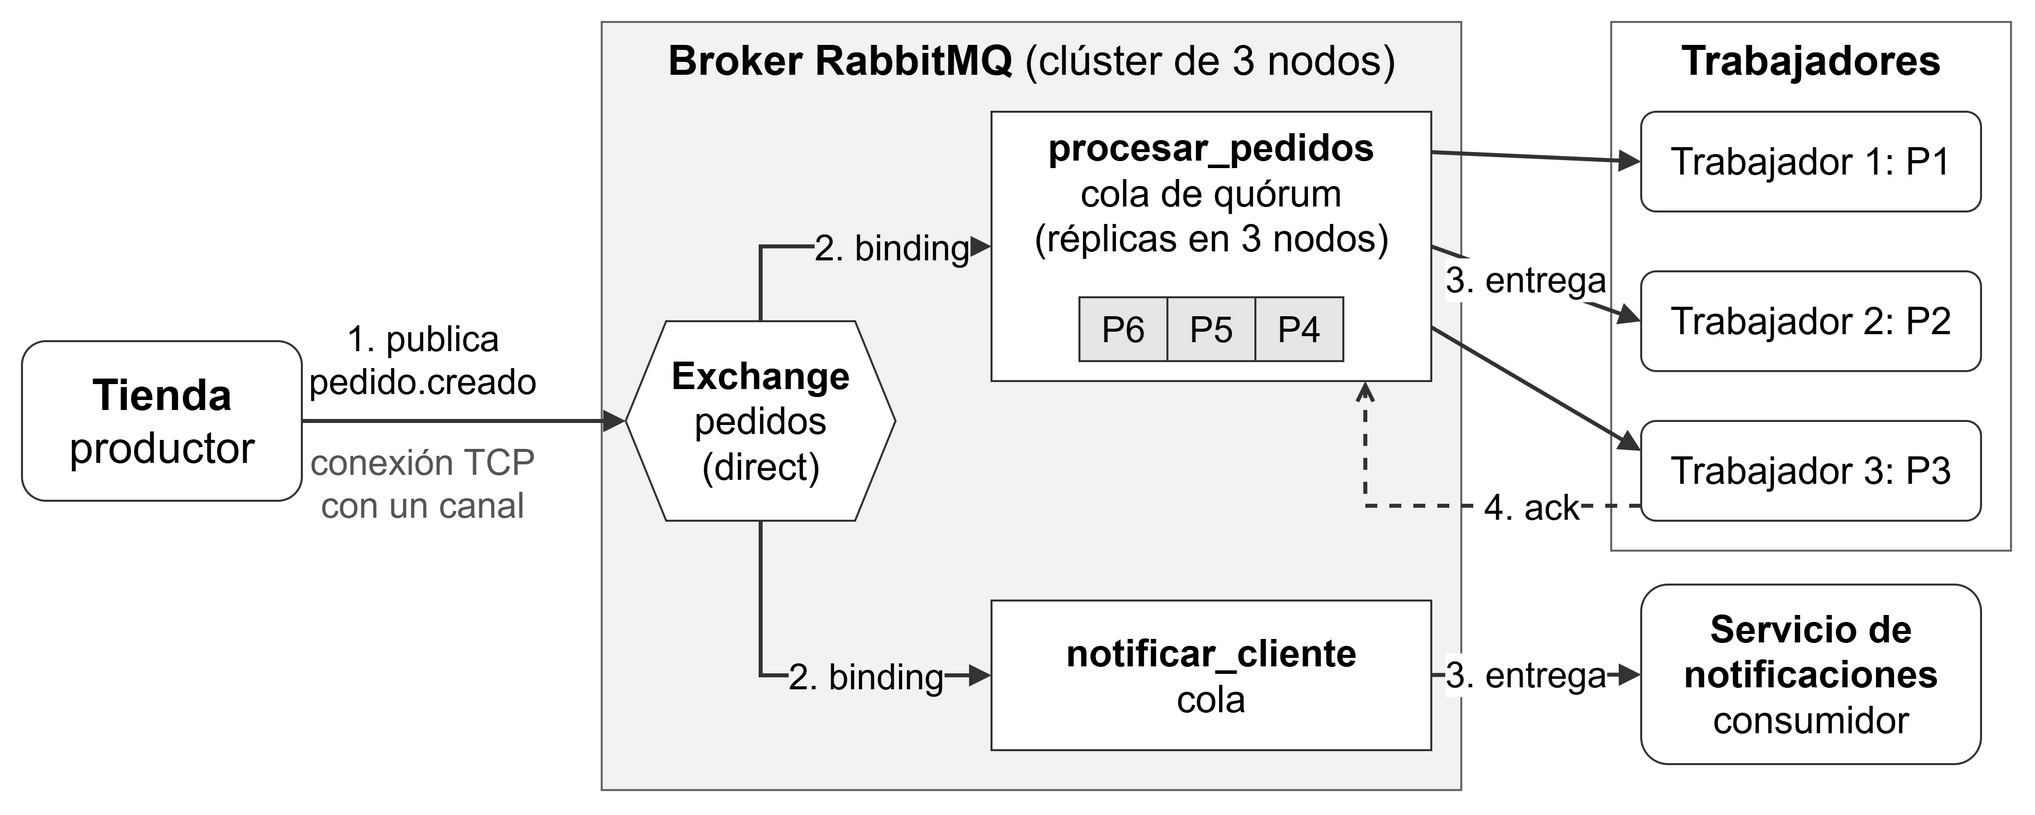
\includegraphics[width=0.85\textwidth]{diagramas/arquitectura.png}
  \caption{Recorrido de un pedido en RabbitMQ. Elaboración propia.}
  \label{fig:arquitectura-rabbitmq}
\end{figure}

\paragraph{9. Transparencias.}
La tienda no sabe qué trabajador ni qué nodo atiende el pedido (ubicación),
la cola replicada se ve como una sola (replicación), los trabajadores la
comparten sin coordinarse (concurrencia) y, si uno cae, su pedido pasa a otro
(fallos) \cite{vansteen2023distributed,rabbitmq2026clustering}.

\paragraph{10. Limitaciones.}
Un pedido reentregado puede procesarse dos veces; si cae un nodo, la tienda
debe reconectarse; con tres nodos la cola de quórum solo tolera un fallo; y la
demora de la red no se oculta \cite{rabbitmq2026queues,rabbitmq2026quorum}.
Estos compromisos se analizan con CAP y PACELC en el apartado siguiente.
